\documentclass{sigchi}

% Use this section to set the ACM copyright statement (e.g. for
% preprints).  Consult the conference website for the camera-ready
% copyright statement.

% Copyright
\CopyrightYear{2019} 
\setcopyright{acmcopyright} 
\conferenceinfo{CHIuXiD'19,}{April 1--9, 2019, Jakarta, Surabaya, Bali, Indonesia}
\isbn{978-1-4503-6187-3/19/04}\acmPrice{\$15.00}
\doi{https://doi.org/10.1145/3328243.3328265}


% Use this command to override the default ACM copyright statement
% (e.g. for preprints).  Consult the conference website for the
% camera-ready copyright statement.

%% HOW TO OVERRIDE THE DEFAULT COPYRIGHT STRIP --
%% Please note you need to make sure the copy for your specific
%% license is used here!
% \toappear{
% Permission to make digital or hard copies of all or part of this work
% for personal or classroom use is granted without fee provided that
% copies are not made or distributed for profit or commercial advantage
% and that copies bear this notice and the full citation on the first
% page. Copyrights for components of this work owned by others than ACM
% must be honored. Abstracting with credit is permitted. To copy
% otherwise, or republish, to post on servers or to redistribute to
% lists, requires prior specific permission and/or a fee. Request
% permissions from \href{mailto:Permissions@acm.org}{Permissions@acm.org}. \\
% \emph{CHI '16},  May 07--12, 2016, San Jose, CA, USA \\
% ACM xxx-x-xxxx-xxxx-x/xx/xx\ldots \$15.00 \\
% DOI: \url{http://dx.doi.org/xx.xxxx/xxxxxxx.xxxxxxx}
% }

% Arabic page numbers for submission.  Remove this line to eliminate
% page numbers for the camera ready copy
% \pagenumbering{arabic}

% Load basic packages
\usepackage{balance}       % to better equalize the last page
\usepackage{graphics}      % for EPS, load graphicx instead 
\usepackage[T1]{fontenc}   % for umlauts and other diaeresis
\usepackage{txfonts}
\usepackage{mathptmx}
\usepackage[pdflang={en-US},pdftex]{hyperref}
\usepackage{color}
\usepackage{booktabs}
\usepackage{textcomp}
\usepackage{verbatim}


% Some optional stuff you might like/need.
\usepackage{microtype}        % Improved Tracking and Kerning
% \usepackage[all]{hypcap}    % Fixes bug in hyperref caption linking
\usepackage{ccicons}          % Cite your images correctly!
% \usepackage[utf8]{inputenc} % for a UTF8 editor only

% If you want to use todo notes, marginpars etc. during creation of
% your draft document, you have to enable the "chi_draft" option for
% the document class. To do this, change the very first line to:
% "\documentclass[chi_draft]{sigchi}". You can then place todo notes
% by using the "\todo{...}"  command. Make sure to disable the draft
% option again before submitting your final document.
\usepackage{todonotes}

\usepackage{tikz}
\def\checkmark{\tikz\fill[scale=0.4](0,.35) -- (.25,0) -- (1,.7) -- (.25,.15) -- cycle;}

% Paper metadata (use plain text, for PDF inclusion and later
% re-using, if desired).  Use \emtpyauthor when submitting for review
% so you remain anonymous.
\def\plaintitle{A Research through Design (Rtd) Approach in the Design of a 360-Video Platform Interface}
\def\plainauthor{Julian de Castro, Emir Mendoza, Brian Poblete, Giselle Nodalo, Jordan Aiko Deja}
\def\emptyauthor{}
\def\plainkeywords{Human Centered Design, User Centered Design, 360 Video, Interface Design}
\def\plaingeneralterms{Guidelines, Design}

% llt: Define a global style for URLs, rather that the default one
\makeatletter
\def\url@leostyle{%
  \@ifundefined{selectfont}{
    \def\UrlFont{\sf}
  }{
    \def\UrlFont{\small\bf\ttfamily}
  }}
\makeatother
\urlstyle{leo}

% To make various LaTeX processors do the right thing with page size.
\def\pprw{8.5in}
\def\pprh{11in}
\special{papersize=\pprw,\pprh}
\setlength{\paperwidth}{\pprw}
\setlength{\paperheight}{\pprh}
\setlength{\pdfpagewidth}{\pprw}
\setlength{\pdfpageheight}{\pprh}

% Make sure hyperref comes last of your loaded packages, to give it a
% fighting chance of not being over-written, since its job is to
% redefine many LaTeX commands.
\definecolor{linkColor}{RGB}{6,125,233}
\hypersetup{%
  pdftitle={\plaintitle},
% Use \plainauthor for final version.
%  pdfauthor={\plainauthor},
  pdfauthor={\emptyauthor},
  pdfkeywords={\plainkeywords},
  pdfdisplaydoctitle=true, % For Accessibility
  bookmarksnumbered,
  pdfstartview={FitH},
  colorlinks,
  citecolor=black,
  filecolor=black,
  linkcolor=black,
  urlcolor=linkColor,
  breaklinks=true,
  hypertexnames=false
}

% create a shortcut to typeset table headings
% \newcommand\tabhead[1]{\small\textbf{#1}}

% End of preamble. Here it comes the document.
\begin{document}

\title{\plaintitle}
\numberofauthors{3}
\author{%
  \alignauthor{Brian Michael Poblete\\
    \affaddr{De La Salle University}\\
    \affaddr{Manila, Philippines}\\
    \email{brian\_poblete@dlsu.edu.ph}}\\
    \alignauthor{Emir Christopher Mendoza\\
    \affaddr{De La Salle University}\\
    \affaddr{Manila, Philippines}\\
    \email{emir\_mendoza@dlsu.edu.ph}}\\ 
    \alignauthor{Julian Paolo De Castro\\
    \affaddr{De La Salle University}\\
    \affaddr{Manila, Philippines}\\
    \email{julian\_decastro@dlsu.edu.ph}}\\
    \alignauthor{Jordan Aiko Deja\\
    \affaddr{De La Salle University}\\
    \affaddr{Manila, Philippines}\\
    \email{jordan.deja@dlsu.edu.ph}}\\
    \alignauthor{Giselle Nodalo\\
    \affaddr{De La Salle University}\\
    \affaddr{Manila, Philippines}\\
    \email{giselle\_nodalo@dlsu.edu.ph}}\\
}

\maketitle
\begin{abstract}
Many video interfaces enable multiple sources of input video in displaying and streaming vital information. Most of these setups can be seen in deployed security systems and observer footage that are usually used for surveillance and crisis monitoring. The motivations of this study includes the use of multiple videos of a single event taken from varying sources in the investigation of a crime. In this study, we consider a crowd-sourced approach to multiple sources of video and aim to design an interface towards multiple possible use-cases. In designing this interface, we performed field studies and on site surveying along with initial user tests to validate our ideas. Research through design was added into the methodology to consider multiple point of views considering varying sources of perspective. Specifically, we catered the design of an initial interface in helping multiple users understand several views from various cameras, angles, and positions. The participants chosen for this study are students who have at least the basic technological ability of using a smartphone and taking a video with it. The results of this study could add to the use cases for 360 videos and video live streams. We intend to extend this study by validating the 360-view and designing an algorithm towards stitching one final view crowd-sourced from multiple cameras and streamers. 
\end{abstract}
\category{H.5.2.}{Information Interfaces and Presentation
  (e.g. HCI)}{User--Centered Design}{}{}
\keywords{\plainkeywords}
\section{Introduction}
Videos are widely-used technologies meant for various purposes. They could be useful for surveillance, security, recreating accidents and even capturing memories according to the works of \cite{zhou2011system, han2012reconstruction, balassanian2014system} With the digital age and the ubiquitous approach to mobile technology, virtually anyone with a mobile phone can capture videos to display a particular object of interest. Mobile phones are also able to gather metadata like location coordinates, duration of video and even lighting scenarios according to the work of \cite{lau2018location}. Some video technologies can even detect and capture in-context objects such as smiles, gait, and other humanly-features. This is one consideration we have applied when doing this study. \\
However these techniques remain underutilized, which could still be implemented in more use-cases. More recently, panoramic technology and other video-stitching technologies have paved the way for the creation of 360-videos, thus improving viewing experiences of users similar to the work of \cite{sula2010system}. These conditions and scenarios have not been fully used for actual use-cases that require multiple and crowd-sourced views. Several use-cases involve concert goers and musical events as seen in the work of \cite{shrestha2010automatic}, observing bystanders while recording footage as seen in the work of \cite{singhal2016you}, and even using dash-cams while driving or using the automobiles as seen in the work of \cite{han2012reconstruction}. These scenarios are simply natural human events and activities that can be augmented with improved 360-video technology. Having been taken from varying angles and positions, a video that contains unique auditory and visual cues regarding human activity are pieces of information that can be collected when these technologies are used. By analyzing the position and angle at which a video was taken, we can potentially help investigators develop a detailed order of events say in a given incident that has transpired. This along many use-cases can benefit from multi-sourced videos that are stitched together to resemble a 360 video. \\
In this paper, we will be discussing the process for designing a usable interface that allows multiple live-streams (also known as streams), to be viewed by a user at the same time. This allows a cohesive viewing experience provided that multiple views and angles of a common and single Point-of-Interest (POI).  In this prototype, it is proposed that we can provide valuable and significant viewing experiences especially on emergency situations where crowds typically respond by capturing a video. In this paper, we demonstrate how we have used Research-through-Design (RtD) as a methodology in designing and validating an interface before proceeding to the latter parts of the research. The framework follows through the Research-through-Design methodology as seen in the works of \cite{deja2018myosl, deja2018flow, deja2018building, tamani2018}. We followed a human-centric approach that had greater emphasis on the users while being able to identify the proper use-cases.  Details on the data gathered, instruments used and an analysis of these results are included. We were able to generate three designs for an interface with the best prototype achieving an above average usability score. The goal of this first phase is to be able to understand the needs of the users in our target use case and be able to come up with the appropriate initial design for the prototype. 
\begin{figure}[t]
    \centering
    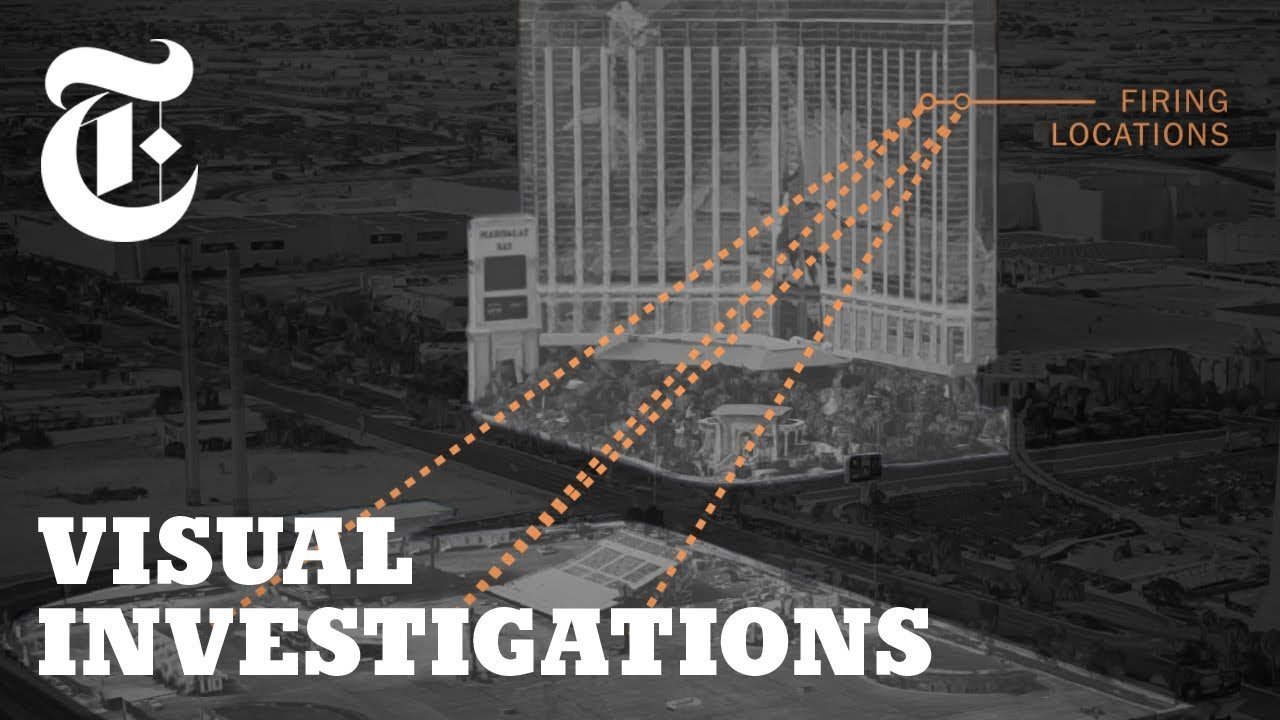
\includegraphics[width = 0.45\textwidth]{figures/lasvegasshooting.jpg}
    \caption{``Screenshot of the Las Vegas Shooting Documentary. In this screenshot we can see how using footage of the event captured from multiple sources paved the way for an easier investigation of the crime scene. A similar but usable approach involving live-streamed video is introduced in this study. Imaged sourced from The New York Times. }
    \label{fig:shooting}
\end{figure}
\begin{figure}[t]
\centering
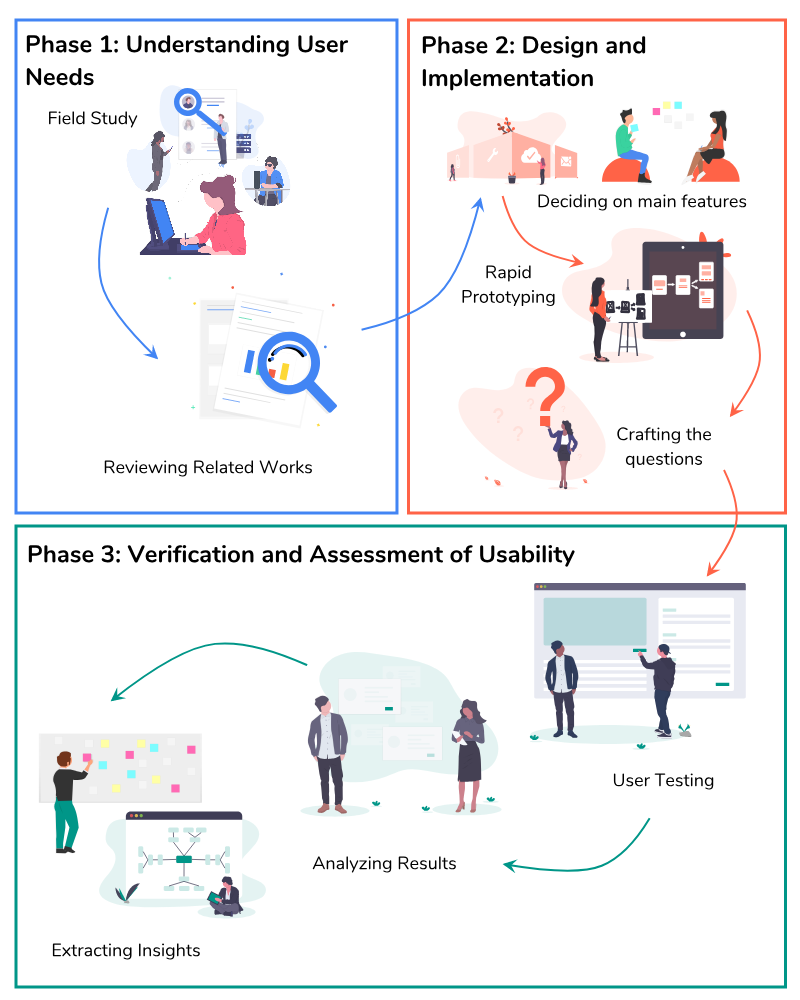
\includegraphics[width = 0.85 \linewidth]{figures/method.png}
\caption{Overview of the three phases in this study. The approach follows a user-centric iterative methodology towards designing an interface. Phase 1 involves a field study and an in-depth analysis of related works in order to devise possible use cases and user needs. Phase 2 includes the development of the prototypes based on the supposed user needs and Phase 3 validates the designs and their features for overall user experience through testing with possible users. }\label{fig:method}
\end{figure}
\section{Related Works}
We have found several studies relating to the key points of our research: The specific keywords revolve around 360-degree video streaming, POI and videos from multiple angles of said points of interest. We considered understanding Points of Interest as our initial scope. We found numerous studies that combine POI along with several concepts like 360-degree video and multiple angles. In the work of \cite{molegi2018regions}, both the area of a user and the areas that a user was previously at was considered in determining the user's next location. These locations have helped a model determine the prediction of the location-based services. Furthermore, the work of \cite{montoliu2013discovering} installed a client-server system on mobile phones, integrating GPS, Wifi, GSM and accelerometer sensors to determine POIs. Our proposal combines technologies similar to these and the usage of videos to provide better perspectives on POIs.\\
In the works of \cite{sheikh2016directing, su2017making, lin2017outside} 360-degree videos have been the focus of developing a software prototype. The study of \cite{sheikh2016directing} focused on subtle and unobtrusive technologies that gave filmmakers and directors methods to direct attention to certain points of the 360-degree video while maintaining the level of control viewers have for the entire duration of the video. Interestingly, in the work of \cite{su2017making}, the same technology was used but this time utilizing an intelligent agent in helping the user find the focus or point of interest. Consequently, in the work of \cite{lin2017outside}, they have enabled technologies of using mini-screens in allowing users find the POI when it is outside the peripheral vision called field of view. These mini-screens were referred to as Picture-in-Picture Previews (PIP). These works consider the different approaches and techniques in allowing the user to find and focus on a particular point of interest. It is interesting to note that these studies enabled flexibility and allowing the user to gain more control and freedom in exploring the interface. There are numerous studies that have worked with 360-degree videos in focus alone or with extracting points of interests in videos alone. The mentioned studies took advantage of utilizing 360-videos as the source of data and using these videos to automatically or dynamically detect a point of interest. In our study, we aim to achieve the opposite of this process, specifically capturing multiple angles and being able to produce a specific point of interest and putting them together in a 360-like video interface. We believe that this approach can pave the way for multiple use-cases to easily extract insights that will be usable in decision making, understanding environments and many others. 
\begin{figure}[t]
    \centering
    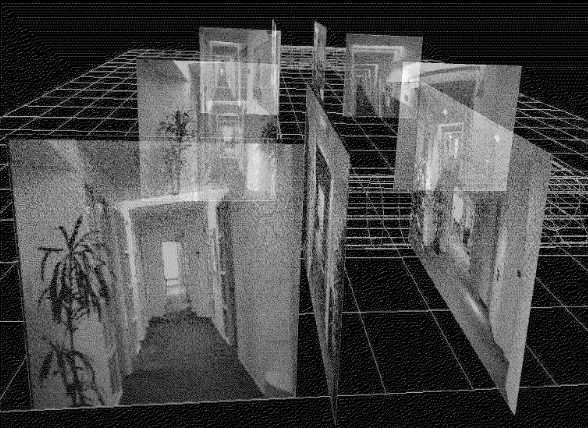
\includegraphics[width = 1\linewidth]{figures/multipleangle.png}
    \caption{A screenshot of a system with multiple cameras used for surveillance systems from the study of \cite{zhou2011system}}
    \label{fig:multiple}
\end{figure}
\section{Methods}
The first phase of this research includes methods the researchers used that are aimed towards understanding how to create a usable interface for the proposed idea. These include taking videos of a certain area from multiple angles simultaneously, Rapid Prototyping, and User-Testing. 

\subsection{Video Taking}
In order to get an idea of how videos of a certain POI could be played simultaneously, we recorded footage in an open-air space from multiple angles at the same time. Mobile cameras were used to record footage while moving the cameras along a set path. After moving a certain distance in a straight line, the cameras were rotated to face one another before moving them in a straight line in a set direction once again. Once the footage had been taken, we analyzed the footage and chose a specific object from the footage as the POI. 

\begin{figure}[t]
    \centering
    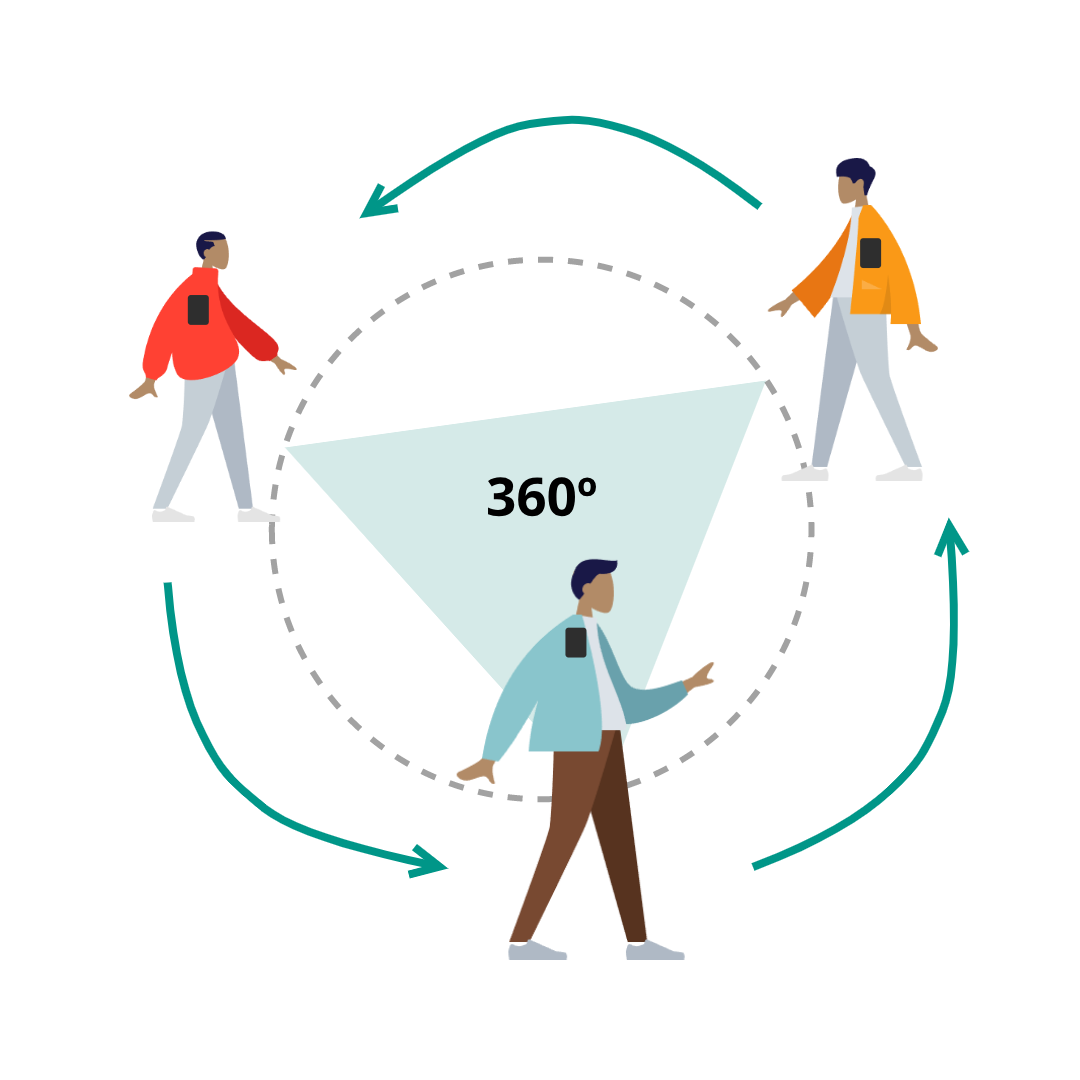
\includegraphics[width = 1\linewidth]{figures/setup.png}
    \caption{A visual representation of the video taking process and field study. The three people placed cameras on their shirt pockets, started recording, and moved along a set path to get a better perspective on the POI from multiple angles. }
    \label{fig:setup}
\end{figure}

\subsection{Rapid Prototyping}
After a POI was chosen, this POI was used as a reference point in designing the prototypes for the application interface. Each of us decided to make one prototype for the interface. In order to devise an interface to display the video streams, we took inspiration from video-streaming sites such as Twitch, YouTube, and Netflix. We then created low-fidelity prototypes to give a basic example of how the videos would be displayed. Afterwards, we created high-fidelity prototypes to give a more concrete sample of the interface. We used Gravit Designer to create the prototype screens and Invision to add interactivity to the screens for user testing.

\subsection{Participants}
Ten (10) undergraduate college students aged 19-20 were recruited through a convenience sampling method. The interviews were scheduled based on the participants' availability and were carried out in a public, indoor space with a high volume of bystanders.


%demographic table

\subsection{Study Design}
% BEFORE THE INTERVIEW
% Describe how interviews were scheduled, where they were interviewed, basically the protocol for the interview. What were the questions, etc. What else did you prepare prior to the interview? Did you give them any form to fill out?

The participants underwent proper research briefing before the actual experiment. They were given consent and waiver forms to ensure proper privacy and handling of data. After the briefing they were free to use the web app as if it was their first time on a brand new website. They were also free to ask the researchers anything they did not understand, provided they tried everything they could to try to understand it without aid. Since there were 3 prototype to be tested, each tester was given a tester number and selected what prototype number they were testing. We used Google Forms as a platform to collect the answers of our testers. Our setup had 2 laptops with one displaying the Form and the other displaying the prototypes. First, we ask for the testers' consent in answering the form through the starting page of the questionnaire. The starting page states the purpose of our data collection and introduces the researchers. Afterwards, they are asked to tick check-boxes corresponding to which personal information they will allow the researchers to use. These include Age, Profession, Civil Status and Sex. The users then filled up the information they wish to provide and filled in their tester number and the prototype they were currently testing. The participant number was mainly used for the convenience of the researchers so we could easily track their responses as they had to submit the form 3 times, 1 for each prototype. 
During the interview, each participant was asked three (3) sets of questions with at least two (2) questions per set. The goal of the first set was to identify the current stand of the participant regarding their experiences in learning about ML and the various tools they have used. The goal of the second set was to identify the various problem areas that the participant associated with based on their experience using current ML tools. The third set was used to identify improvements regarding usability of the tool, as pointed out by the participant. The questions that were used are as follows:
        \begin{itemize}
            \item Upon first glance of this website I was able to determine that this page uses multiple points of view.
            \item With prolonged usage I was able to determine that this page uses multiple points of view.
            \item Upon first glance of this website I was able to see through the map that there is a P.O.I. in the area.
            \item With prolonged usage I was able to see through the map that there is a P.O.I. in the area.
            \item How well can you see the POI from different points of view?
            \item How well can you see the POI in "Mesh Mode"?
            \item How did you find navigating through the website? Why? 
            \item How did you find switching from different points of view? Why? 
            \item How well were you able to understand what each of the hotspots do by just looking at them, or clicking on them once? Why? 
            \item How fast were you able to get used to the navigation of this website?
            \item I was able to understand completely the functions of the system. 
        \end{itemize}

The participants answered items 1 to 4 following a 4-point Likert scale with 1 being Strongly Disagree and 4 being Strongly Agree. These focused on determining whether a POI could be easily identified and viewed from multiple angles through the interface or not. The second set of questions (Items 5 and 6) focused on the clarity of the POI. These questions used a 4-point Likert scale with 1 being Very Unclear and 4 being Very Clearly. The last set of questions focused on the usability of the interface. The questions used 4-point Likert scales accompanied by open-ended questions for the participant to explain why they gave that rating. We also asked them to suggest ways to improve functions they did not understand in the event that they find such functions. We utilized descriptive statistical analysis to obtain the mean of the participants' responses to the questions and the mode of their responses. The open-ended follow-up questions enabled us to use the narrative analysis method for the qualitative data.

% AFTER THE INTERVIEW
\subsection{Limitations}
These methods used for our research include several limitations. Regarding video taking, we simulated the streaming of a POI from multiple angles by systematically recording a POI from multiple angles. However, we could not simulate 360 video streaming as we had no access to a 360 camera and thus could not design for a display that accounts for a 360 video stream. For the study design, the user tests were conducted in a location convenient for the participants. The location was not the most optimal area for conducting user testing due to it being a public area with various distractions present. Additionally, the usability testing of the prototypes could be executed by testing the prototypes in a random order. Doing so could negate biases caused by testing one prototype before the others.

\section{Results}
This section contains the results from the user tests and the outcomes of the different prototype versions we prepared. Analysis of the figures are presented in mean values are followed by insights. 

\subsection{Prototype Features}
Each prototype features a minimap, a button to activate mesh mode, different screens to view the different points of view and the ability to view in fullscreen the different POV's. Prototype 1 has a navigation bar at the top of the page, the very noticeable "Activate Mesh Mode" button in the middle of the screen and the ability to see what streaming service or social media is being used in each point of view. Prototype 2 has unique labels for each point of view on the top left corner of each screen as well as a label for each point of view on the minimap. Prototype 3 has an interface for Augmented Reality, a scrollable field to browse other events and streams and the ability to click the icons of the other points of view on the main screen. These prototypes are meant for web. Another version will be designed separately for mobile use.

\begin{figure}[h]
    \centering
    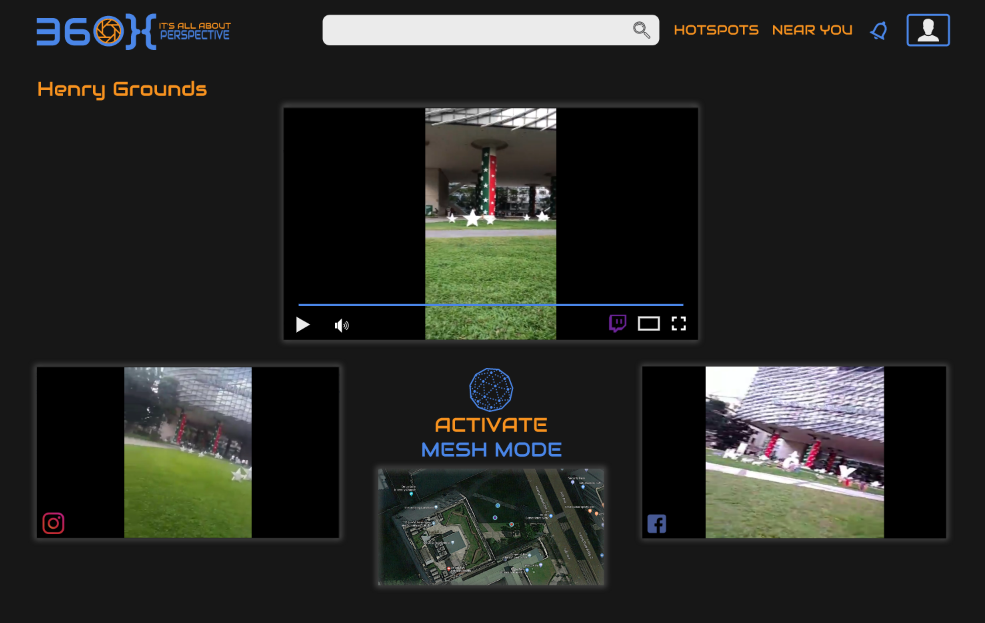
\includegraphics[width = 1\linewidth]{figures/Prototype_1.png}
    \caption{Prototype 1. This prototype shows the different angles, in this case 3 angles, of the streamed POI. In the middle of the screen is a button to activate "Mesh Mode". The navigation bar on the top of the page enables the users to easily move around the website, featuring a "Hotspots" button, a "Near You" button, and a "Home" button which is found on the top left corner. It also shows a minimap on the middle bottom of the screen.}
    \label{fig:multiple}
\end{figure}
\begin{figure}[h]
    \centering
    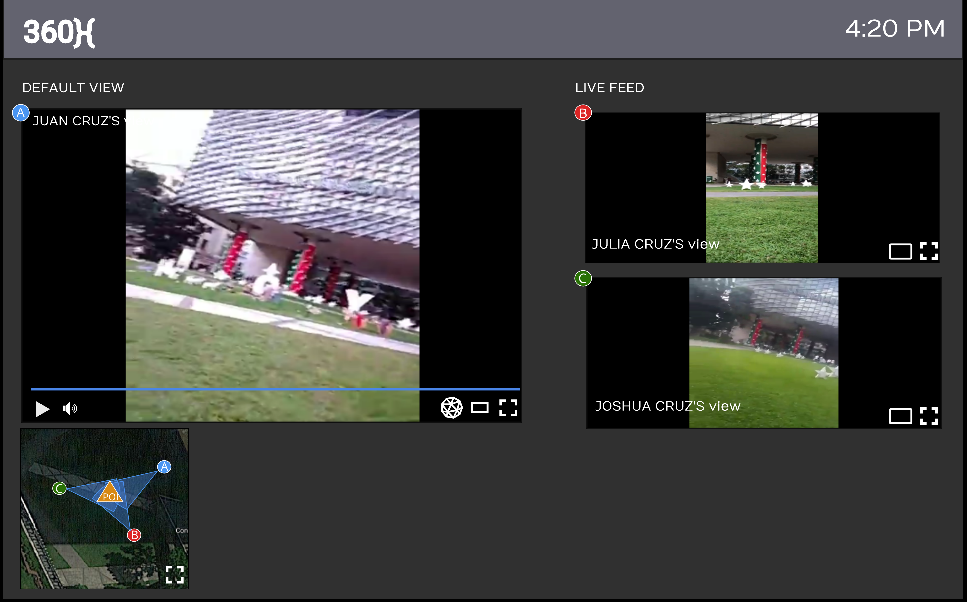
\includegraphics[width = 1\linewidth]{figures/Prototype_2.png}
    \caption{Prototype 2. This prototype shows the different angles on a POI with a main angle being displayed on the left side. The right side shows other angles of the view. Each view angle is indicated on the minimap located on the bottom left of the screen. The minimap indicates the positions of the different view angles (represented by alphabetical letters) as well as the position of the POI (represented by the triangular icon).}
    \label{fig:multiple}
\end{figure}

\begin{figure}[h]
    \centering
    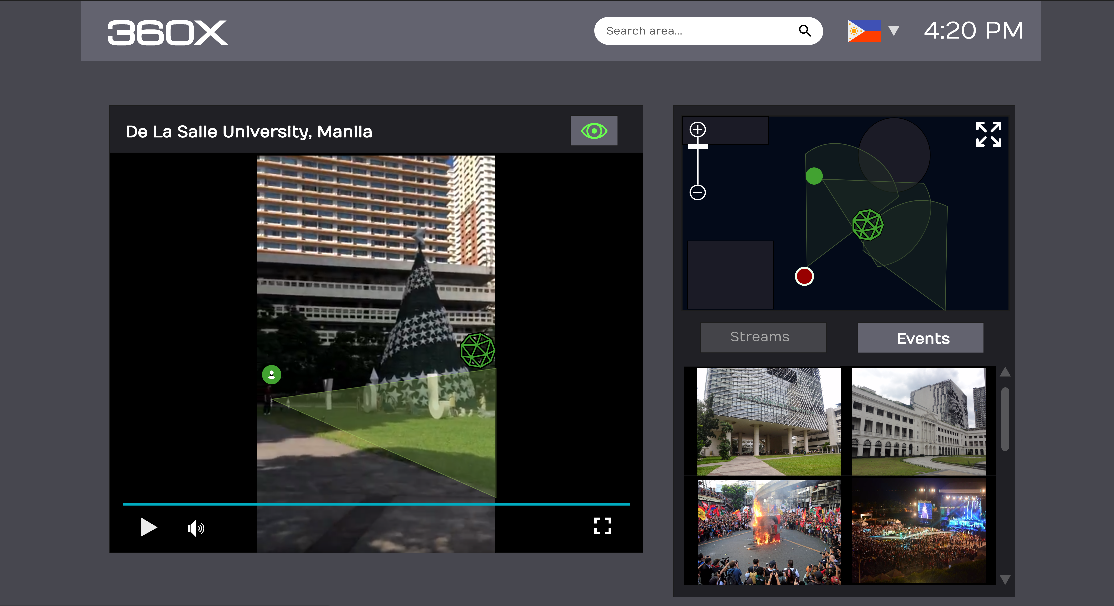
\includegraphics[width = 1\linewidth]{figures/Prototype_3.png}
    \caption{Prototype 3. This prototype has multiple ways to switch between the angles of a POI. In the video player to the left, other people streaming the POI will be highlighted and their field of view will be shown. On the upper right corner, a minimap is shown for an overhead view of the area and POI. The lower right corner will display in a list the different POIs in the area under the events tab and the different people streaming the current POI.}
    \label{fig:multiple}
\end{figure}
\newpage
\subsection{User Feedback and Insights}
%% HI BRIAN INSERT ANALYSIS HERE 
Table 1 indicates that Prototype 3 fared the best in each criterion (Focus, Clarity, Usability). Participants generally liked the easy-to-use design of the prototype. They described the use of icons and images as intuitive and understandable. On the other hand, Prototype 2 had the lowest score for each criterion. This was due mainly to the vagueness of the buttons used and the lack of basic functions such as a back or home button.
%%What is it in the features of Prototype X that made it the best in Y? or worst in Z?

% What were the common qualitative statements that describes each prototype? 

\begin{table}[h]
\centering
\caption{Table of average scores for each prototype for each criteria.}
\begin{tabular}{|l|l|l|l|l}
\cline{1-4}
            & \textbf{Focus} & \textbf{Clarity} & \textbf{Usability}   \\ \cline{1-4}
\textbf{P1} & 3.5            & 3.1              & 3.2                  \\ \cline{1-4}
\textbf{P2} & 3.1           & 2.9              & 2.7                 \\ \cline{1-4}
\textbf{P3} & 3.6           & 3.6              & 3.4                  \\ \cline{1-4}
\end{tabular}
\end{table}
% Insights on the averages
It can be observed on the table of averages that the best prototype version is Prototype 3. It garnered a score of 3.5, a few notches higher than Prototype 1 and Prototype 2. In terms of managing focus while using the interface, Prototype 3 scored the highest. However, there are still minor areas for improvement for Prototype 3 in terms of usability, specifically on overall navigation and switching from different points of view. It can also be observed that Prototype 2 scored the lowest especially on the areas of Navigation, understandability of the hotspots upon glances and on determining the POI through a minimap. By analyzing the individual scores for each areas, it is interesting to note that all prototypes scored relatively higher on the criteria of being able to view the POI with multiple angles from prolonged usage. This means that all three versions of the prototype where built for long periods of use. 

\begin{table}[h]
\centering
\caption{Results of the Initial Usability Test done on the three (3) Prototypes. Each area segment concentrated on Focus, Clarity and Usability.}
\begin{tabular}{|l|r|r|r|}
\hline
                                                                     & \textbf{Prototype 1}  & \textbf{Prototype 2}  & \textbf{Prototype 3}  \\ \hline
\textbf{Focus}                                                       &              &              &              \\ \hline
Q1                                                                   & 3.0            & 3.1          & 3.3          \\ \hline
Q2                                                                   & 4.0            & 3.6          & 4            \\ \hline
Q3                                                                   & 3.3          & 2.6          & 3.4          \\ \hline
Q4                                                                   & 3.7          & 3.3          & 3.9          \\ \hline
\textbf{Clarity}                                                     &              &              &              \\ \hline
Q5                                                                   & 3.2          & 3.1          & 3.7          \\ \hline
Q6                                                                   & 3.0            & 2.7          & 3.5          \\ \hline
\textbf{Usability}                                                   &              &              &              \\ \hline
Q7                                                                   & 3.0            & 2.3          & 3.1          \\ \hline
Q8                                                                   & 3.5          & 3.1          & 3.1          \\ \hline
Q9                                                                   & 2.8          & 2.5          & 3.4          \\ \hline
Q10                                                                  & 3.2          & 2.8          & 3.4          \\ \hline
Q11                                                                  & 3.5          & 3.2          & 3.7          \\ \hline
\textbf{\begin{tabular}[c]{@{}l@{}}Prototype\\ Average\end{tabular}} & \textbf{3.2} & \textbf{2.9} & \textbf{3.5} \\ \hline
\end{tabular}
\end{table}


% Understanding outputs from current tools they use 

 

\subsection{Comparisons to Previous Studies}
We compared the results of this study to previous research findings mentioned by analyzing the main features of prototype 3 and similar features found in the other works. First, the work of \cite{zhou2011system} details a navigation interface that allows a user to view video streams captured from multiple angles in a 3-D immersive environment, in comparison, our interface allows the user to view these multiple angles through a 360-degree video instead. Another basis of comparison would be the work of \cite{shrestha2010automatic} where they collect recordings of multiple angles of concerts. Instead of collecting recordings of events, our interface would be able to compile live streams of on-going events and allow the user to switch between them in real time. In the work of \cite{molegi2018regions} they were able to collect the locations and interests from their users' smartphones to generate multiple POI. Our work is able to collect and compile our users' real-time camera feed and location and generate POI from that data.


%% HELLO JULIAN IM HERE 
%% HALLO
\section{Conclusion and Future Work}
We have designed and developed prototypes to provide an interface for the concept of viewing a POI from multiple angles. This was made possible by Research-through-Design and by enabling a user-centric approach in our methodology.  This generates a 360-degree video using the data from these angles. The features implemented were inspired from the Las Vegas shooting aforementioned and other related works. To validate the usability of these prototypes, we had these prototypes evaluated and the results analyzed from our data collection and gathered insights from our participants. We also noted other studies on using location data to generate POIs, improving the user experience of 360-degree videos and their implementations. Our research combines various aspects of these papers to create a flexible crowd-sourced system. For our future work in this project, our second phase will further validate the 360-view following the design of the Prototype 3 as it had the highest average with all of its aspects having the best mean scores. The third phase will involve designing an algorithm that aims to stitch together multiple video streams into one coherent view using a specialized algorithm.

\section{Acknowledgments}
We would like to thank De La Salle University College of Computer Studies and the Center for Complexity and Emerging Technologies for all the support that they have given us. We would also like to thank the testers and respondents who sacrificed their time for our interaction study. We would also like to thank Prof. Anthony Tang for the inspiration behind this study. 

% Balancing columns in a ref list is a bit of a pain because you
% either use a hack like flushend or balance, or manually insert
% a column break.  http://www.tex.ac.uk/cgi-bin/texfaq2html?label=balance
% multicols doesn't work because we're already in two-column mode,
% and flushend isn't awesome, so I choose balance.  See this
% for more info: http://cs.brown.edu/system/software/latex/doc/balance.pdf
%
% Note that in a perfect world balance wants to be in the first
% column of the last page.
%
% If balance doesn't work for you, you can remove that and
% hard-code a column break into the bbl file right before you
% submit:
%
% http://stackoverflow.com/questions/2149854/how-to-manually-equalize-columns-
% in-an-ieee-paper-if-using-bibtex
%
% Or, just remove \balance and give up on balancing the last page.
%
\balance{}

%\section{References Format}
%Your references should be published materials accessible to the
%public. Internal technical reports may be cited only if they are
%easily accessible and may be obtained by any reader for a nominal
%fee. Proprietary information may not be cited. Private communications
%should be acknowledged in the main text, not referenced (e.g.,
%[Golovchinsky, personal communication]). References must be the same
%font size as other body text. References should be in alphabetical
%order by last name of first author. Use a numbered list of references
%at the end of the article, ordered alphabetically by last name of
%first author, and referenced by numbers in brackets. For papers from
%conference proceedings, include the title of the paper and the name of
%the conference. Do not include the location of the conference or the
%exact date; do include the page numbers if available. 

%References should be in ACM citation format:
%\url{http://www.acm.org/publications/submissions/latex_style}.  This
%includes citations to Internet
%resources~\cite{CHINOSAUR:venue,cavender:writing,psy:gangnam}
%according to ACM format, although it is often appropriate to include
%URLs directly in the text, as above. Example reference formatting for
%individual journal articles~\cite{ethics}, articles in conference
%proceedings~\cite{Klemmer:2002:WSC:503376.503378},
%books~\cite{Schwartz:1995:GBF}, theses~\cite{sutherland:sketchpad},
%book chapters~\cite{winner:politics}, an entire journal
%issue~\cite{kaye:puc},
%websites~\cite{acm_categories,cavender:writing},
%tweets~\cite{CHINOSAUR:venue}, patents~\cite{heilig:sensorama}, 
%games~\cite{supermetroid:snes}, and
%online videos~\cite{psy:gangnam} is given here.  See the examples of
%citations at the end of this document and in the accompanying
%\texttt{BibTeX} document. This formatting is a edited version of the
%format automatically generated by the ACM Digital Library
%(\url{http://dl.acm.org}) as ``ACM Ref.'' DOI and/or URL links are
%optional but encouraged as are full first names. Note that the
%Hyperlink style used throughout this document uses blue links;
%however, URLs in the references section may optionally appear in
%black.

% BALANCE COLUMNS
\balance{}

% REFERENCES FORMAT
% References must be the same font size as other body text.
\bibliographystyle{SIGCHI-Reference-Format}
\bibliography{sample}

\end{document}

%%% Local Variables:
%%% mode: latex
%%% TeX-master: t
%%% End:
